\chapter{Mediciones de Aplicaciones} \label{ch:measurements}

% **************************** Define Graphics Path **************************
\ifpdf
    \graphicspath{{Chapter5/Figs/Raster/}{Chapter5/Figs/PDF/}{Chapter5/Figs/}}
\else
    \graphicspath{{Chapter5/Figs/Vector/}{Chapter5/Figs/}}
\fi

En este capítulo se realizan diferentes tipos de mediciones de aplicación. El mismo se encuentra dividido en dos secciones, la primera trata sobre ensayos aplicados en el simulador, para estudiar el efecto de la utilización de un objeto externo para la medición de la distancia entre el radar y el objeto a medir. La segunda sección resume los resultados obtenidos de las mediciones tomadas con el radar sobre un portafolios metálico.


\section{Mediciones con Simulador}

En esta sección se realizan dos tipos de mediciones de aplicación con el simulador, representadas en la figura \ref{fig:DistDependencySim}. Se puede observar que la distancia entre el mezclador y el blanco es la distancia real sumada a un delta de distancia, el cual entre ensayo y ensayo se variará para obtener resultados. La primer medición toma al delta como valores conocidos, en cambio para la segunda, es tratada como una incertidumbre de medición.
\begin{figure}
  \centering
  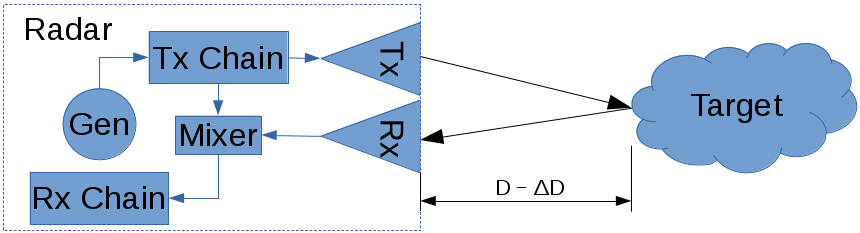
\includegraphics[width=12cm]{distanceDependency}
  \caption{Medición de propiedades del blanco ante diferentes deltas de distancias.}
  \label{fig:DistDependencySim}
\end{figure}


\subsection{Dependencia con distancia}

En esta sección se estudia la dependencia de la medición de los parámetros S del blanco iluminado con respecto a un error en la determinación de la distancia. Este ensayo es para determinar el efecto de utilizar un componente externo para medir el rango entre el blanco y el radar, y como el mismo no estaría en la posición del mezclador, se estaría introduciendo este tipo de error sistemático. 

La tabla \ref{tab:simDeltaDist} resume los resultados obtenidos. La columna Error indica el valor adoptado en la variable delta de la figura \ref{fig:DistDependencySim}. En otras palabras, sería a cuantos metros más cerca del blanco está el medidor de distancia con respecto al mezclador.

\begin{table}[htb]
  \caption{Parámetros S del blanco a distintas distancias utilizando el simulador.}
  \centering
  \label{tab:simDeltaDist}
  \begin{tabular}{l *{4}{S[table-auto-round, table-format=-1.2] S[table-auto-round, table-format=-3.2]}}
  \toprule
  \multirow{4}{1cm}{\textbf{Delta [m]}} & \multicolumn{8}{c}{\textbf{Distancia [m]}} \tabularnewline
  \cmidrule{2-9}
   & \multicolumn{2}{c}{30760} & \multicolumn{2}{c}{35000} & \multicolumn{2}{c}{37760.1695} & \multicolumn{2}{c}{40000} \tabularnewline
  \cmidrule(r){2-3} \cmidrule(lr){4-5} \cmidrule(lr){6-7} \cmidrule(l){8-9}
   & {Gain} & {Phase} & {Gain} & {Phase} & {Gain} & {Phase} & {Gain} & {Phase} \tabularnewline
   & [$\si{\deci\bel}$] & [$\si{\deg}$] & [$\si{\deci\bel}$] & [$\si{\deg}$] & [$\si{\deci\bel}$] & [$\si{\deg}$] & [$\si{\deci\bel}$] & [$\si{\deg}$] \tabularnewline
  \midrule
  
  0 & 0.9974998783 & -0.8999873159 & 0.9970854521 & 5.0829022535 & 0.9974244573 & 0.0563536612 & 0.9991246271 & 1.1021289469 \tabularnewline

  5 & 0.996851467 & -28.5141663823 & 0.9965158111 & -22.5305974732 & 0.9968962677 & -27.5567038267 & 0.9986251585 & -26.5105696718 \tabularnewline

  10 & 0.9962033718 & -56.1283462497 & 0.9959464141 & -50.1440980009 & 0.9963682879 & -55.1697621157 & 0.9981258771 & -54.1232690916 \tabularnewline

  40 & 0.9923214343 & 138.1865577226 & 0.9925351551 & 144.1748820091 & 0.9932048122 & 139.1518713272 & 0.9951341194 & 140.2005175668 \tabularnewline

  100 & 0.984591606 & 166.8162791476 & 0.9857389337 & 172.8127555094 & 0.986900466 & 167.7950516932 & 0.9891707856 & 168.8480043635 \tabularnewline

  \bottomrule 
  \end{tabular}
\end{table}

Se puede observar que la variación en el resultado para la determinación de la ganancia es despreciable, en cambio, para la fase es totalmente determinante. Cabe destacar que una separación entre el mezclador y el medidor de $\SI{5}{\meter}$ implica que la señal recorre $\SI{10}{\meter}$ menos, dado que la misma recorre el mismo camino dos veces. A su vez, independientemente de la distancia a la que está el blanco, un error igual a $\SI{5}{\meter}$ implica un desfase igual a $\SI{-27.61}{\deg}$. Este resultado es el esperado dado que la longitud de onda de la señal transmitida es aproximadamente $\SI{122}{\meter}$, por lo tanto un error de $\SI{12.2}{\meter}$ implica un desfase de $\SI{36}{\deg}$.

La figura \ref{fig:deltaDistSim} muestra de forma separada las mediciones de la ganancia y fase del blanco en las distancias $\SI{30760}{\meter}$, $\SI{35000}{\meter}$, $\SI{37760.1695}{\meter}$ y $\SI{40000}{\meter}$.
\begin{figure}[H]
  \centering
  \begin{subfigure}{0.49\textwidth}
    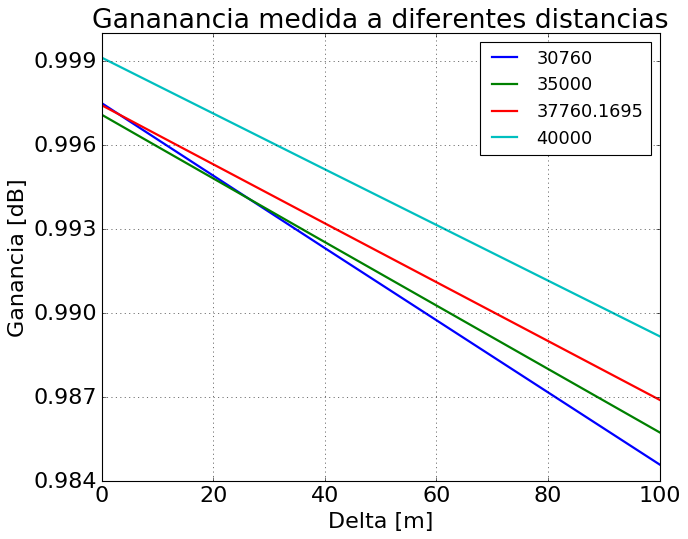
\includegraphics[width=7cm]{deltaDistGain}
    \caption{Ganancia}
  \end{subfigure}
  \begin{subfigure}{0.49\textwidth}
    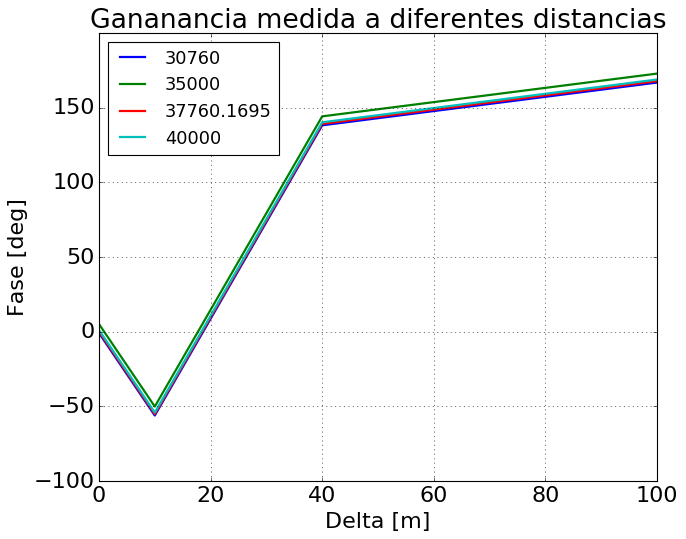
\includegraphics[width=7cm]{deltaDistPhase}
    \caption{Fase}
  \end{subfigure}
  \caption{Parámetros S del blanco a distintas distancias.}
  \label{fig:deltaDistSim}
\end{figure}

\subsection{Incertidumbre en distancia}

En esta sección se introducen incertidumbres en la medición de la distancia buscando determinar cómo afecta a la medición de los parámetros S del blanco iluminado. Dichas incertidumbres se las toma con distribución gaussiana con desvío estándar configurable y media igual a cero. La tabla \ref{tab:simIncertDist} resume los resultados obtenidos de la simulación de montecarlo con 1000 realizaciones.

\begin{table}[htb]
  \caption{Parámetros S del blanco a distintas distancias.}
  \centering
  \label{tab:simIncertDist}
  \begin{tabular}{l *{4}{S[table-auto-round, table-format=-1.2] S[table-auto-round, table-format=-3.2]}}
  \toprule
  \multirow{4}{1cm}{\textbf{Std [m]}} & \multicolumn{8}{c}{\textbf{Distancia [m]}} \tabularnewline
  \cmidrule{2-9}
   & \multicolumn{2}{c}{30760} & \multicolumn{2}{c}{35000} & \multicolumn{2}{c}{37760.1695} & \multicolumn{2}{c}{40000} \tabularnewline
  \cmidrule(r){2-3} \cmidrule(lr){4-5} \cmidrule(lr){6-7} \cmidrule(l){8-9}
   & {Gain} & {Phase} & {Gain} & {Phase} & {Gain} & {Phase} & {Gain} & {Phase} \tabularnewline
   & [$\si{\deci\bel}$] & [$\si{\deg}$] & [$\si{\deci\bel}$] & [$\si{\deg}$] & [$\si{\deci\bel}$] & [$\si{\deg}$] & [$\si{\deci\bel}$] & [$\si{\deg}$] \tabularnewline
  \midrule
  
  0 & 0.00 & 0.00 & 0.00 & 0.00 & 0.00 & 0.00 & 0.00 & 0.00 \tabularnewline

  5 & 0.000369507 & 15.7325843211 & 0.0003330912 & 16.1431290009 & 0.0002977873 & 15.5648756904 & 0.0002884168 & 15.9418570692 \tabularnewline

  10 & 0.0007337078 & 31.239336556 & 0.0006511433 & 31.5574962315 & 0.0006150956 & 32.1497974883 & 0.0005796089 & 32.0371315787 \tabularnewline

  40 & 0.0029849535 & 116.5644598149 & 0.002650077 & 116.673494049 & 0.0023426065 & 112.3447856255  & 0.0023238051 & 117.0437670382 \tabularnewline

  \bottomrule 
  \end{tabular}
\end{table}

Se puede observar que la variación en el resultado para la determinación de la ganancia es despreciable, en cambio, para la fase es totalmente determinante. Cabe destacar que la incertidumbre obtenida no depende de la distancia a la que se encuentra el blanco con respecto al radar.

La figura \ref{fig:incertDistSim} muestra la dependencia lineal entre la incertidumbre de la medición de la fase del blanco y el desvío estándar de la distancia al cual se encuentra. Se puede observar que si se desea no tener una incertidumbre absoluta mayor a $\SI{30}{\degree}$, no se debe tener una incertidumbre en la distancia mayor a $\SI{8.33}{\meter}$.
\begin{figure}[H]
  \centering
  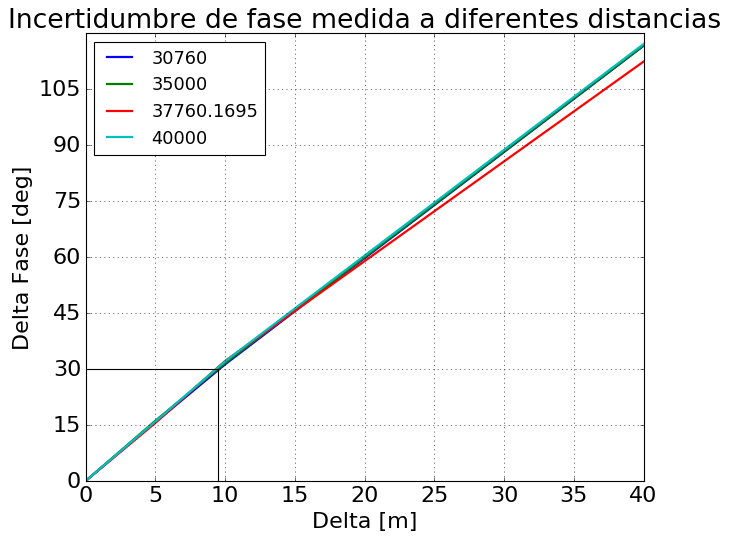
\includegraphics[width=9cm]{incertDistPhase}
  \caption{Medición de fase del blanco ante diferentes incertidumbres en distancias.}
  \label{fig:incertDistSim}
\end{figure}


\section{Mediciones con Radar}

En esta sección se realizan dos tipos de mediciones de aplicación con el radar utilizando como blanco a un portafolios frente a paneles absorvedores para disminuir los ecos en las paredes de la sala. El esquema de trabajo se encuentra representado en la figura \ref{fig:DistDependencySim2}. Se puede observar que la distancia entre el mezclador y el blanco es la distancia real sumada a un delta de distancia, el cual entre ensayo y ensayo, se variará para obtener resultados. Para la primer medición el delta es conocido, en cambio para la segunda, es tratado como una incertidumbre de medición y se lo mantuvo invariante.
\begin{figure}[htb]
  \centering
  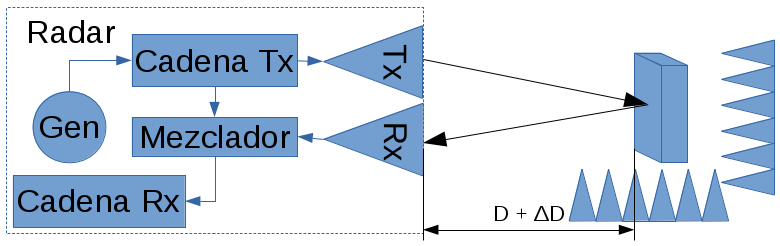
\includegraphics[width=12cm]{distanceDependencyRadar}
  \caption{Medición de propiedades de un portafolios ante diferentes deltas de distancias.}
  \label{fig:DistDependencySim2}
\end{figure}

La figura \ref{fig:radarMeasurement} muestra el momento y el ambiente en que la medición tomó lugar.
\begin{figure}[htb]
  \centering
  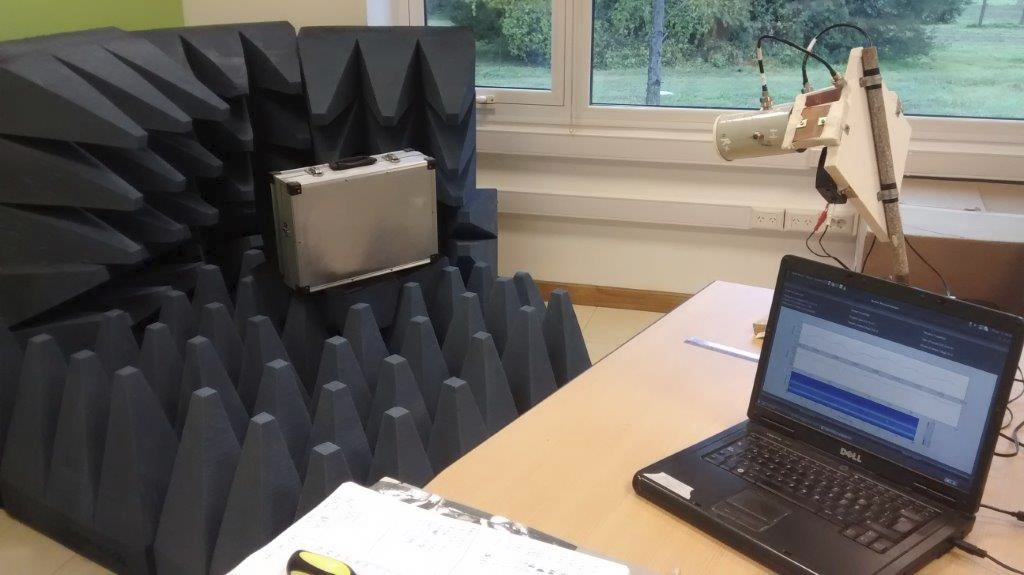
\includegraphics[width=12cm]{radarMeasurement}
  \caption{Medición de propiedades de un portafolios con el radar.}
  \label{fig:radarMeasurement}
\end{figure}


\subsection{Dependencia con distancia}

En esta sección se estudia la dependencia de la medición de los parámetros S del blanco iluminado con respecto a un error en la determinación de la distancia. Este ensayo es para determinar el efecto de utilizar un componente externo para medir el rango entre el blanco y el radar, y como el mismo no estaría en la posición del mezclador, se estaría introduciendo este tipo de error sistemático.

La tabla \ref{tab:simDeltaDistRadar} resume los resultados obtenidos. La columna Error indica el valor adoptado en la variable delta de la figura \ref{fig:DistDependencySim2}. En otras palabras, sería a cuantos metros más cerca del blanco está el medidor de distancia con respecto al mezclador.

\begin{table}[htb]
  \caption{Parámetros S del blanco a distintas distancias utilizando el radar.}
  \centering
  \label{tab:simDeltaDistRadar}
  \begin{tabular}{l *{3}{S[table-auto-round, table-format=-1.2] S[table-auto-round, table-format=-3.2]}}
  \toprule
  \multirow{4}{1cm}{\textbf{Delta [$\si{\milli\meter}$]}} & \multicolumn{6}{c}{\textbf{Distancia [$\si{\meter}$]}} \tabularnewline
  \cmidrule{2-7}
   & \multicolumn{2}{c}{1.71} & \multicolumn{2}{c}{1.84} & \multicolumn{2}{c}{2.005} \tabularnewline
  \cmidrule(r){2-3} \cmidrule(lr){4-5} \cmidrule(l){6-7}
   & {Gain} & {Phase} & {Gain} & {Phase} & {Gain} & {Phase} \tabularnewline
   & [$\si{\dB}$] & [$\si{\deg}$] & [$\si{\dB}$] & [$\si{\deg}$] & [$\si{\dB}$] & [$\si{\deg}$] \tabularnewline
  \midrule
  
  0 & 81.464 & -174.1 & 81.654 & 57.2 & 82.18 & 5 \tabularnewline

  5 & 80.947 & 100.3 & 81.175 & -28.4 & 82.14 & 32.4 \tabularnewline

  10 & 80.417 & 14.7 & 80.677 & -114 & 82.104 & 60 \tabularnewline

  15 & 79.873 & -70.9 & 80.17 & 160.3 & 82.063 & 87.4 \tabularnewline

  \bottomrule 
  \end{tabular}
\end{table}

Se puede observar que la variación en el resultado para la determinación de la ganancia no resulta despreciable dado que al haber $\SI{15}{\milli\meter}$ de diferencia la medición disminuyó en $\SI{1.591}{\dB}$ y para el caso de la fase es totalmente determinante. Cabe destacar que una separación entre el mezclador y el medidor de $\SI{5}{\milli\meter}$ implica que la señal recorre $\SI{10}{\milli\meter}$ menos, dado que la misma recorre el mismo camino dos veces. A su vez, independientemente de la distancia a la que está el blanco, un error igual a $\SI{5}{\milli\meter}$ implica un desfase igual a $\SI{27.6}{\deg}$. Este resultado es el esperado dado que la longitud de onda de la señal transmitida es aproximadamente $\SI{122}{\milli\meter}$, por lo tanto un error de $\SI{12.2}{\meter}$ implica un desfase de $\SI{36}{\deg}$.

\begin{figure}[H]
  \centering
  \begin{subfigure}{0.49\textwidth}
    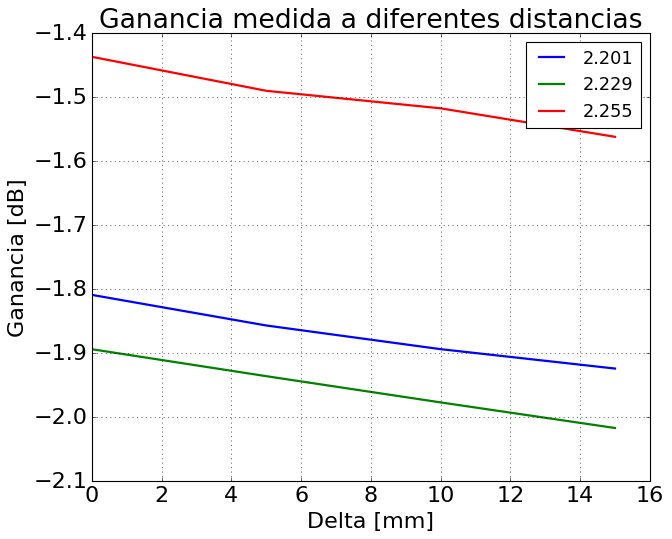
\includegraphics[width=7cm]{deltaDistGainRadar}
    \caption{Ganancia}
  \end{subfigure}
  \begin{subfigure}{0.49\textwidth}
    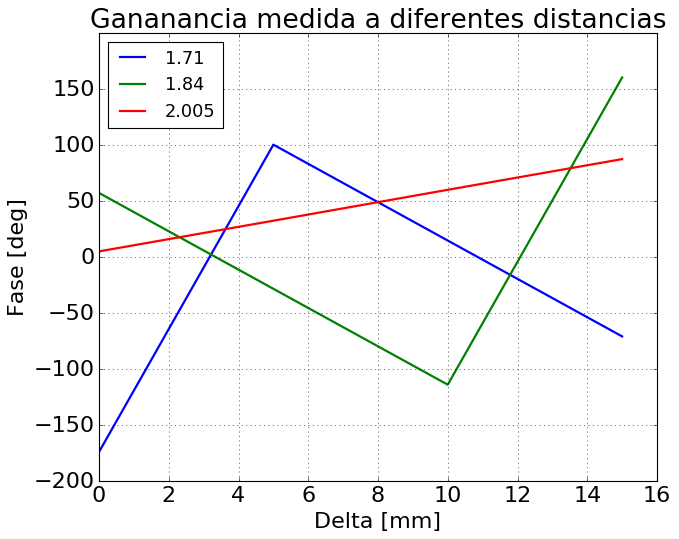
\includegraphics[width=7cm]{deltaDistPhaseRadar}
    \caption{Fase}
  \end{subfigure}
  \caption{Parámetros S del blanco a distintas distancias.}
  \label{fig:deltaDistRadar}
\end{figure}
La figura \ref{fig:deltaDistRadar} muestra de forma separada las mediciones de la ganancia y fase del blanco en las distancias $\SI{1.71}{\meter}$, $\SI{1.84}{\meter}$ y $\SI{2.005}{\meter}$. Se puede observar que para las distancias menores la variación de ganancia es mucho mayor que a la máxima medida, esto se atribuye a una mayor influencia de los lóbulos secundarios del crosstalk sobre las mismas. Se puede apreciar lo mismo ante la variación de fase.


\subsection{Mediciones a diferentes distancias}

En esta sección se realizan diferentes mediciones variando la distancia al cuerpo para ver si hay variaciones en la determinación de los parámetros S del blanco iluminado. Se escojen dos tipos de blancos, un maletin y un corner reflector.

\subsubsection{Medición de un maletín}

La tabla \ref{tab:radarMeasurementResults} resume los resultados obtenidos. El error absoluto detallado es la distancia de tres desvíos estándar dado que se tomó la hipótesis de estar trabajando con una incertidumbre con distribución gaussiana.

\begin{table}[H]
  \caption{Parámetros S del portafolios medidos con el radar.}
  \centering
  \label{tab:radarMeasurementResults}
  \begin{tabular}{c c S[table-auto-round, table-format=-2.2] S[table-auto-round, table-format=1.2] S[table-auto-round, table-format=-3] S[table-auto-round, table-format=2]}
  \toprule
  \textbf{Distancia [m]} & \textbf{Polarización} & \textbf{Gain [$\si{\deci\bel}$]} & \textbf{$\Delta$Gain [$\si{\deci\bel}$]} & \textbf{Phase [$\si{\deg}$]} & \textbf{$\Delta$Phase [$\si{\deg}$]} \tabularnewline
  \midrule
  
  \multirow{4}{*}{1.32} & HH & 71.1565 & 0.0675 & -106.8 & 18.2 \tabularnewline
   & HV & 60.5657 & 0.0882 & -15.0 & 19.7 \tabularnewline
   & VH & 60.5657 & 0.0882 & -140.8 & 34.4 \tabularnewline
   & VV & 64.8014 & 0.1615 & -165.1 & 37.2 \tabularnewline

  \cmidrule{2-6}
  \multirow{4}{*}{1.56} & HH & 68.9655 & 0.0762 & -163.2 & 30.0 \tabularnewline
   & HV & 60.2654 & 0.1644 & 68.4 & 22.6 \tabularnewline
   & VH & 60.2654 & 0.1644 & -95.4 & 17.2 \tabularnewline
   & VV & 81.8009 & 0.1089 & -179.3 & 32.3 \tabularnewline

  \cmidrule{2-6}
  \multirow{4}{*}{1.71} & HH & 71.2909 & 0.0802 & 28.1 & 27.0 \tabularnewline
   & HV & 54.8529 & 0.2380 & 137.9 & 11.8 \tabularnewline
   & VH & 58.5789 & 0.0963 & 50.5 & 21.0 \tabularnewline
   & VV & 81.7132 & 0.1219 & 25.4 & 46.2 \tabularnewline

  \cmidrule{2-6}
  \multirow{4}{*}{1.84} & HH & 85.9835 & 0.0500 & 80.7 & 33.8 \tabularnewline
   & HV & 52.2837 & 0.1081 & 72.0 & 13.8 \tabularnewline
   & VH & 56.1397 & 0.1092 & -162.4 & 27.8 \tabularnewline
   & VV & 85.2886 & 0.0840 & -150.4 & 39.5 \tabularnewline

  \cmidrule{2-6}
  \multirow{4}{*}{2.005} & HH & 69.2779 & 0.0746 & 18.1 & 19.2 \tabularnewline
   & HV & 52.3194 & 0.1185 & 10.3 & 14.5 \tabularnewline
   & VH & 54.9835 & 0.0557 & 122.9 & 14.9 \tabularnewline
   & VV & 82.2477 & 0.0464 & -97.5 & 23.3 \tabularnewline

  \bottomrule
  \end{tabular}
\end{table}
\todo{cambiar tabla}

Se puede observar en la tabla \ref{tab:radarMeasurementResults} una gran variación entre mediciones de ganancia de la misma polarización a diferentes distancias. Esto se debe a que no se tomó en cuenta que el control del volumen de la computadora estaba en modo automático, por lo tanto entre ensayo y ensayo se modificó su nivel de ganancia, introduciendo un error grosero en dicha magnitud. De todas formas se puede sacar como conclusión que el portafolios posee una gran atenuación ante las polarizaciones cruzadas con respecto a las co-polares, la cual puede llegar a ser $\SI{27}{\dB}$ menor. A su vez se observa una tendencia de mayor ganancia para las polarizaciones verticales que para las horizontales. Para la estimación de fase no parece ser consistente entre ensayos realizados por lo tanto no es concluyente.


\subsubsection{Medición de un Corner Reflector}

Para esta experiencia se construye un corner reflector triangular de $\SI{50}{\centi\meter}$ de lado, ver figura \ref{fig:corner}. El máximo RCS que se puede obtener, siguiendo la ecuación \ref{eq:theoreticalRcs}, es igual a $\SI{12.43}{\dB}$. Luego de su construcción, se midieron el ángulo de cada cara y se observa que poseen $\SI{88.5}{\deg}$, esto implica que el eco recibido debería estar disminuído en $\SI{10}{\dB}$, ver figura \ref{fig:cornerErrors}.
\begin{figure}[htb]
  \centering
  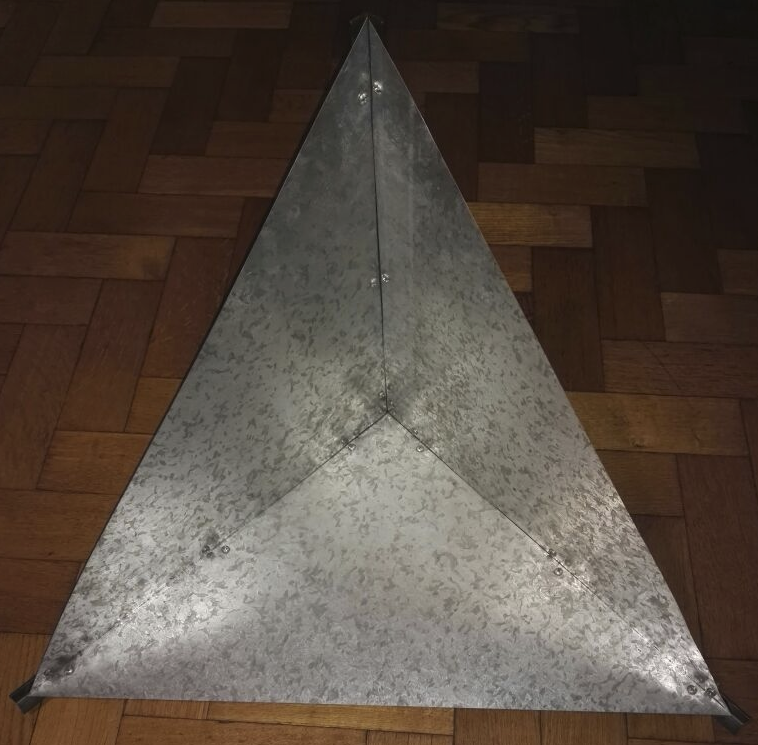
\includegraphics[width=6cm]{cornerReflector}
  \caption{Corner reflector construído de $\SI{50}{\centi\meter}$ de lado para realizar las mediciones.}
  \label{fig:corner}
\end{figure}
La tabla \ref{tab:cornerMeasurementResults} resume los resultados obtenidos. El error absoluto detallado es la distancia de tres desvíos estándar dado que se tomó la hipótesis de estar trabajando con una incertidumbre con distribución gaussiana.

\begin{table}[H]
  \caption{Parámetros S del corner reflector medidos con el radar.}
  \centering
  \label{tab:cornerMeasurementResults}
  \begin{tabular}{c c S[table-auto-round, table-format=-2.2] S[table-auto-round, table-format=1.2] S[table-auto-round, table-format=-3] S[table-auto-round, table-format=2]}
  \toprule
  \textbf{Distancia [m]} & \textbf{Polarización} & \textbf{Gain [$\si{\deci\bel}$]} & \textbf{$\Delta$Gain [$\si{\deci\bel}$]} & \textbf{Phase [$\si{\deg}$]} & \textbf{$\Delta$Phase [$\si{\deg}$]} \tabularnewline
  \midrule

  \multirow{4}{*}{1.32} & HH & 71.1565 & 0.0675 & -106.8 & 18.2 \tabularnewline
   & HV & 60.5657 & 0.0882 & -15.0 & 19.7 \tabularnewline
   & VH & 60.5657 & 0.0882 & -140.8 & 34.4 \tabularnewline
   & VV & 64.8014 & 0.1615 & -165.1 & 37.2 \tabularnewline

  \cmidrule{2-6}
  \multirow{4}{*}{1.56} & HH & 68.9655 & 0.0762 & -163.2 & 30.0 \tabularnewline
   & HV & 60.2654 & 0.1644 & 68.4 & 22.6 \tabularnewline
   & VH & 60.2654 & 0.1644 & -95.4 & 17.2 \tabularnewline
   & VV & 81.8009 & 0.1089 & -179.3 & 32.3 \tabularnewline

  \cmidrule{2-6}
  \multirow{4}{*}{1.71} & HH & 71.2909 & 0.0802 & 28.1 & 27.0 \tabularnewline
   & HV & 54.8529 & 0.2380 & 137.9 & 11.8 \tabularnewline
   & VH & 58.5789 & 0.0963 & 50.5 & 21.0 \tabularnewline
   & VV & 81.7132 & 0.1219 & 25.4 & 46.2 \tabularnewline

  \cmidrule{2-6}
  \multirow{4}{*}{1.84} & HH & 85.9835 & 0.0500 & 80.7 & 33.8 \tabularnewline
   & HV & 52.2837 & 0.1081 & 72.0 & 13.8 \tabularnewline
   & VH & 56.1397 & 0.1092 & -162.4 & 27.8 \tabularnewline
   & VV & 85.2886 & 0.0840 & -150.4 & 39.5 \tabularnewline

  \cmidrule{2-6}
  \multirow{4}{*}{2.005} & HH & 69.2779 & 0.0746 & 18.1 & 19.2 \tabularnewline
   & HV & 52.3194 & 0.1185 & 10.3 & 14.5 \tabularnewline
   & VH & 54.9835 & 0.0557 & 122.9 & 14.9 \tabularnewline
   & VV & 82.2477 & 0.0464 & -97.5 & 23.3 \tabularnewline

  \bottomrule
  \end{tabular}
\end{table}
\todo{cambiar tabla}

\section{Resumen}

En este capítulo se realizaron mediciones de aplicación tanto con el simulador como con el radar.

Con el simulador se estudió la dependencia del resultado ante errores en la determinación de la distancia y ante incertidumbres en la misma. Para el primer caso la determinación de la ganancia es casi invariante, en cambio para la fase se puede observar que ante diferencias de distancia de $\lambda / 10$ se observan desfases de $\SI{36}{\degree}$. Para el segundo caso, se repiten los mismos resultados dado que si se desea tener una incertidumbre menor a $\SI{36}{\degree}$, se debe tener una incertidumbre menor a $\lambda / 10$ en la determinación de la distancia.

Con el radar se realizaron ensayos de la dependencia del resultado ante errores en la determinación de la distancia y se midió de mismo blanco a distintas distancias. Para el primer caso, solamente se observa el resultado esperado en la determinación de la ganancia y fase para una distancia mínima de $\SI{2}{\meter}$, para distancias menores se debe evitar realizar mediciones dado que los lóbulos secundarios del cross-talk entre las antenas interfieren la medición.